\documentclass[conference]{IEEEtran}
\IEEEoverridecommandlockouts
\usepackage{cite}
\usepackage{amsmath,amssymb,amsfonts}
\usepackage{algorithmic}
\usepackage{graphicx}
\usepackage{textcomp}
\usepackage{xcolor}
\def\BibTeX{{\rm B\kern-.05em{\sc i\kern-.025em b}\kern-.08em
    T\kern-.1667em\lower.7ex\hbox{E}\kern-.125emX}}
\begin{document}

\title{Enforcing Contextual Integrity at the Information Type: Measuring
Over-Delivery in Document-Level Access Control}

\author{\IEEEauthorblockN{1\textsuperscript{st} Ryan Thornton}
\IEEEauthorblockA{\textit{Dept. of Computer Science} \\
\textit{Tennessee Technological University}\\
Cookeville, TN, USA \\
rthornton42@tntech.edu}
\and
\IEEEauthorblockN{2\textsuperscript{nd} Manaak Gupta}
\IEEEauthorblockA{\textit{Dept. of Computer Science} \\
\textit{Tennessee Technological University}\\
Cookeville, TN, USA \\
email address or ORCID}
\and
\IEEEauthorblockN{3\textsuperscript{rd} Mir Pritom}
\IEEEauthorblockA{\textit{Dept. of Computer Science} \\
\textit{Tennessee Technological University}\\
Cookeville, TN, USA \\
email address or ORCID}
}

\maketitle

\begin{abstract}
Contextual Integrity defines appropriate information flow over information
types: a diagnosis, a salary figure, an insurance identifier. Deployed access
control enforces over objects, releasing or refusing a document whole. A
document correctly released therefore delivers every type it happens to carry,
including types the recipient has no business holding. We measure that gap.
Extending a deterministic Contextual Integrity gate that mediates document
retrieval for a language-model agent, we add a fifth conjoined check requiring
the subject-linked information types a document carries to be a subset of those
the requester's role may receive. Supporting the check requires an inventory the
system does not have, so we build and audit one: a 16-entry controlled
vocabulary, a domain tagger measured at 0.994 precision and 1.000 recall over
400 annotated cells on a corpus five of its rules were revised against, and a
per-occurrence subject-linkage classifier measured at 0.955 precision on
filtered classes over 487 annotated detections. Reconciling the extracted
inventory against the hand-authored labels, no document of 105 matches exactly
and 520 document-type pairs are present but unlabelled. Six role permission sets
were authored by hand rather than by a model, since prior work finds language
models unable to author normative policy reliably. Re-adjudicating all 2520
flows, the check converts 81 of 259 permits to denials with zero over-blocks
across the 600 flows where ground truth exists, and the role field and the type
check prove non-redundant in both directions. The check also renders 67 of 105
documents reachable by nobody: specification-first labelling produces documents
whose contents exceed what any admitted role may lawfully receive. A derived
bound predicts that result to within one document. The mechanism generalizes;
the magnitude does not.
\end{abstract}

\begin{IEEEkeywords}
contextual integrity, access control, privacy, large language models, retrieval
\end{IEEEkeywords}

\section{Introduction}

Contextual Integrity \cite{b1}, \cite{b2} holds that a flow of information is
appropriate when it conforms to the norms of the context in which the
information originated. The theory is defined over a five-tuple of sender,
recipient, subject, information type, and transmission principle, and the
information type is load-bearing. A diagnosis shared with a treating physician
is appropriate; the same diagnosis shared with a billing clerk is not, even
though both are employees of the same clinic and both are entitled to see
records about that patient.

Systems do not enforce at that granularity. Access control mediates objects: a
file, a record, a document is released or it is not. When an object is released,
everything printed on it goes with it. A billing specialist who correctly
receives an insurance claim also receives the diagnosis code printed on that
claim, the patient's date of birth, their home address, and, in the corpus
studied here, frequently their Social Security Number. No access-control list
resolves this, because the label has no vocabulary for ``this document minus the
diagnosis''.

This is not a novel observation. Object-level versus attribute-level granularity
is long-settled ground in access control \cite{b3}. What is missing is
measurement: how much information does object-level enforcement actually
over-deliver on a system whose policy is otherwise correct? And what happens
when the finer-grained check is added? Does it close the gap, at what cost in
false denials, and does it subsume the coarser check or complement it?

We answer those questions on a deterministic Contextual Integrity gate that
mediates document retrieval for a language-model agent \cite{b4}. The gate reads
only the requester's role, context, and assignments together with the document's
label; it never reads document content. It reproduces its specification on all
2520 requester-document flows of a 105-document synthetic clinic corpus. We
extend it with a fifth conjoined check,
\begin{equation}
\{\, t : t \in T(d) \wedge \mathrm{subj}(t,d) \,\} \subseteq P(\mathrm{role}(r)),
\label{eq:check}
\end{equation}
where $T(d)$ is the set of information types document $d$ carries,
$\mathrm{subj}(t,d)$ holds when occurrence $t$ concerns the document's subject,
and $P(\cdot)$ is a role's permission set, so that access becomes a three-term
intersection of role, assignment, and information type.

The check requires an input the system does not have. The label schema carries
an attribute field, and prior work maps it to the Contextual Integrity
information-type parameter, but files it under provenance and never consults it
at decision time. We first establish what that field would have to contain, and
how far it can be trusted, before making the gate read it.

The contributions are as follows. First, a measurement of over-delivery under
document-level enforcement: 81 of 259 permitted flows carry information types the
recipient's role may not receive, attributed to the responsible type, role, and
sensitivity tier. Second, an audited extraction pipeline, comprising a
controlled vocabulary, a domain tagger, and a subject-linkage classifier, each
with human ground truth and reported error bounds, including the error direction
that fails silently. Third, a reconciliation showing that hand-authored labels
state a document's purpose rather than enumerate its contents, with 0 of 105
documents matching exactly. Fourth, an ablation measuring what the role field
and the type check each uniquely contribute, rather than asserting that they
differ. Fifth, a limit result: 67 of 105 documents become reachable by no one,
with a derived bound that predicts the figure to within one document and
identifies bundle size as the governing parameter.

\section{Background and Related Work}

\subsection{Contextual Integrity}
Nissenbaum's framework \cite{b1} was formalized by Barth et al. \cite{b2} in a
temporal logic over flows, and has since been applied to survey instruments
\cite{b5}, connected devices \cite{b6}, and normative analysis of platform
behaviour \cite{b7}. The framework rests on a century of doctrinal groundwork
\cite{b8}, and its operationalization remains difficult precisely because the
information-type parameter has no natural machine representation.

\subsection{Privacy and language-model agents}
Language models memorize and reproduce training data \cite{b9}, and retrieval
augmentation \cite{b10} moves the risk from weights to the retrieval channel.
Agentic systems that call tools \cite{b11}, \cite{b12} enlarge the surface
further \cite{b13}, and prompt injection makes the model's own judgement an
unreliable guard \cite{b14}, \cite{b15}. Benchmarks now probe whether models
reason about contextual norms \cite{b16}, \cite{b17}; the consistent finding is
that they do so unreliably. This motivates architectures that do not ask the
model to \cite{b18}, \cite{b19}. If the model is treated as trust-equivalent to
the requester and the retrieval tool is gated deterministically, confidentiality
becomes a property of the channel rather than of the model's alignment.

\subsection{Granularity in access control}
Role-based access control \cite{b3} and its descendants mediate objects and
operations. Attribute-based access control generalizes this by making decisions
over attributes of subject, object, action, and environment
\cite{b20}, and policy languages such as XACML \cite{b21} express such
rules directly. That attribute-level policy is more expressive than object-level
policy is therefore well established, and we do not claim otherwise. Indeed our
ablation in Section~\ref{sec:overlap} shows the object-level role field uniquely
blocks 100 flows the attribute check does not catch, so the two are
complementary rather than ordered.

The distinction we draw is narrower and, we think, underexamined. ABAC reasons
about attributes \emph{of} an object --- its classification, owner, or age ---
whereas the check studied here reasons about the information types \emph{inside}
it. An object's attributes are metadata a system already holds; the types it
contains must be extracted, and extraction is fallible in ways that metadata is
not. Much of this paper is consequently about establishing how far that
extraction can be trusted before any policy is applied to it, which is a problem
ABAC does not have and a cost its expressiveness result does not price.

Purpose-based access control \cite{b22} and Hippocratic databases
\cite{b23} come closer, binding data use to declared purpose and
attaching retention and disclosure rules at the column level. Both assume a
relational store where the granular unit is already delimited by the schema. The
setting here is documents, where the unit is not delimited at all: an insurance
claim is one object whose contents span five information types, and no column
boundary separates them.

\subsection{De-identification and data minimization}
An alternative response to over-delivery is to remove the offending content
rather than refuse the document. Statutory de-identification under the health
privacy rule enumerates identifiers to strip, and automated de-identification of
clinical narrative has been studied since the i2b2 shared tasks \cite{b24};
formal privacy models such as $k$-anonymity \cite{b25} quantify what
remains after suppression and generalization. These are complementary to our
setting rather than alternatives to it. De-identification rewrites content and
therefore requires reading it, which is precisely what the gated architecture
forbids of its decision path, and it targets re-identification risk rather than
contextual appropriateness: a diagnosis correctly attributed to a patient is not
de-identifiable without destroying the document's clinical purpose, yet it
remains inappropriate for a billing specialist to receive. Our contribution is
the measurement of the gap on a system whose object-level policy is already
correct, and the limit result that follows, which is precisely where redaction
would have to take over.

\subsection{Benchmarks and normative authorship}
PrivaCI-Bench \cite{b26} and GoldCoin \cite{b27} derive Contextual Integrity
flows from court cases interpreting health privacy law, providing label
authority external to any one research group. Prior work in this line \cite{b4}
evaluated language models as authors of the normative policy itself and found
conformance as low as 23 percent with self-agreement as low as 26 percent. That
finding directly constrains the present work: the role permission sets central
to \eqref{eq:check} are authored by hand, as described in
Section~\ref{sec:authoring}. A model-authored permission set would refute the
result it depends on.

\section{System Under Study}

\subsection{Corpus}
The corpus models a fictional clinic: 105 documents across 21 document types,
six populated sensitivity tiers, and 24 agents holding six roles, namely Doctor,
Nurse, Billing Specialist, HR Manager, IT Contractor, and Patient. The cross
product gives 2520 requester-document flows. Each document carries a label
recording its type, originating context, sensitivity tier, subject, permitted
receiver roles, and a governing transmission principle.

Crucially, the corpus was built specification-first: each label was authored by
hand, and content was then generated to satisfy it. Any value in the attribute
field is therefore a specification of what should be present, not an inventory
of what is. Section~\ref{sec:recon} measures the difference.

\begin{figure*}[t]
\centerline{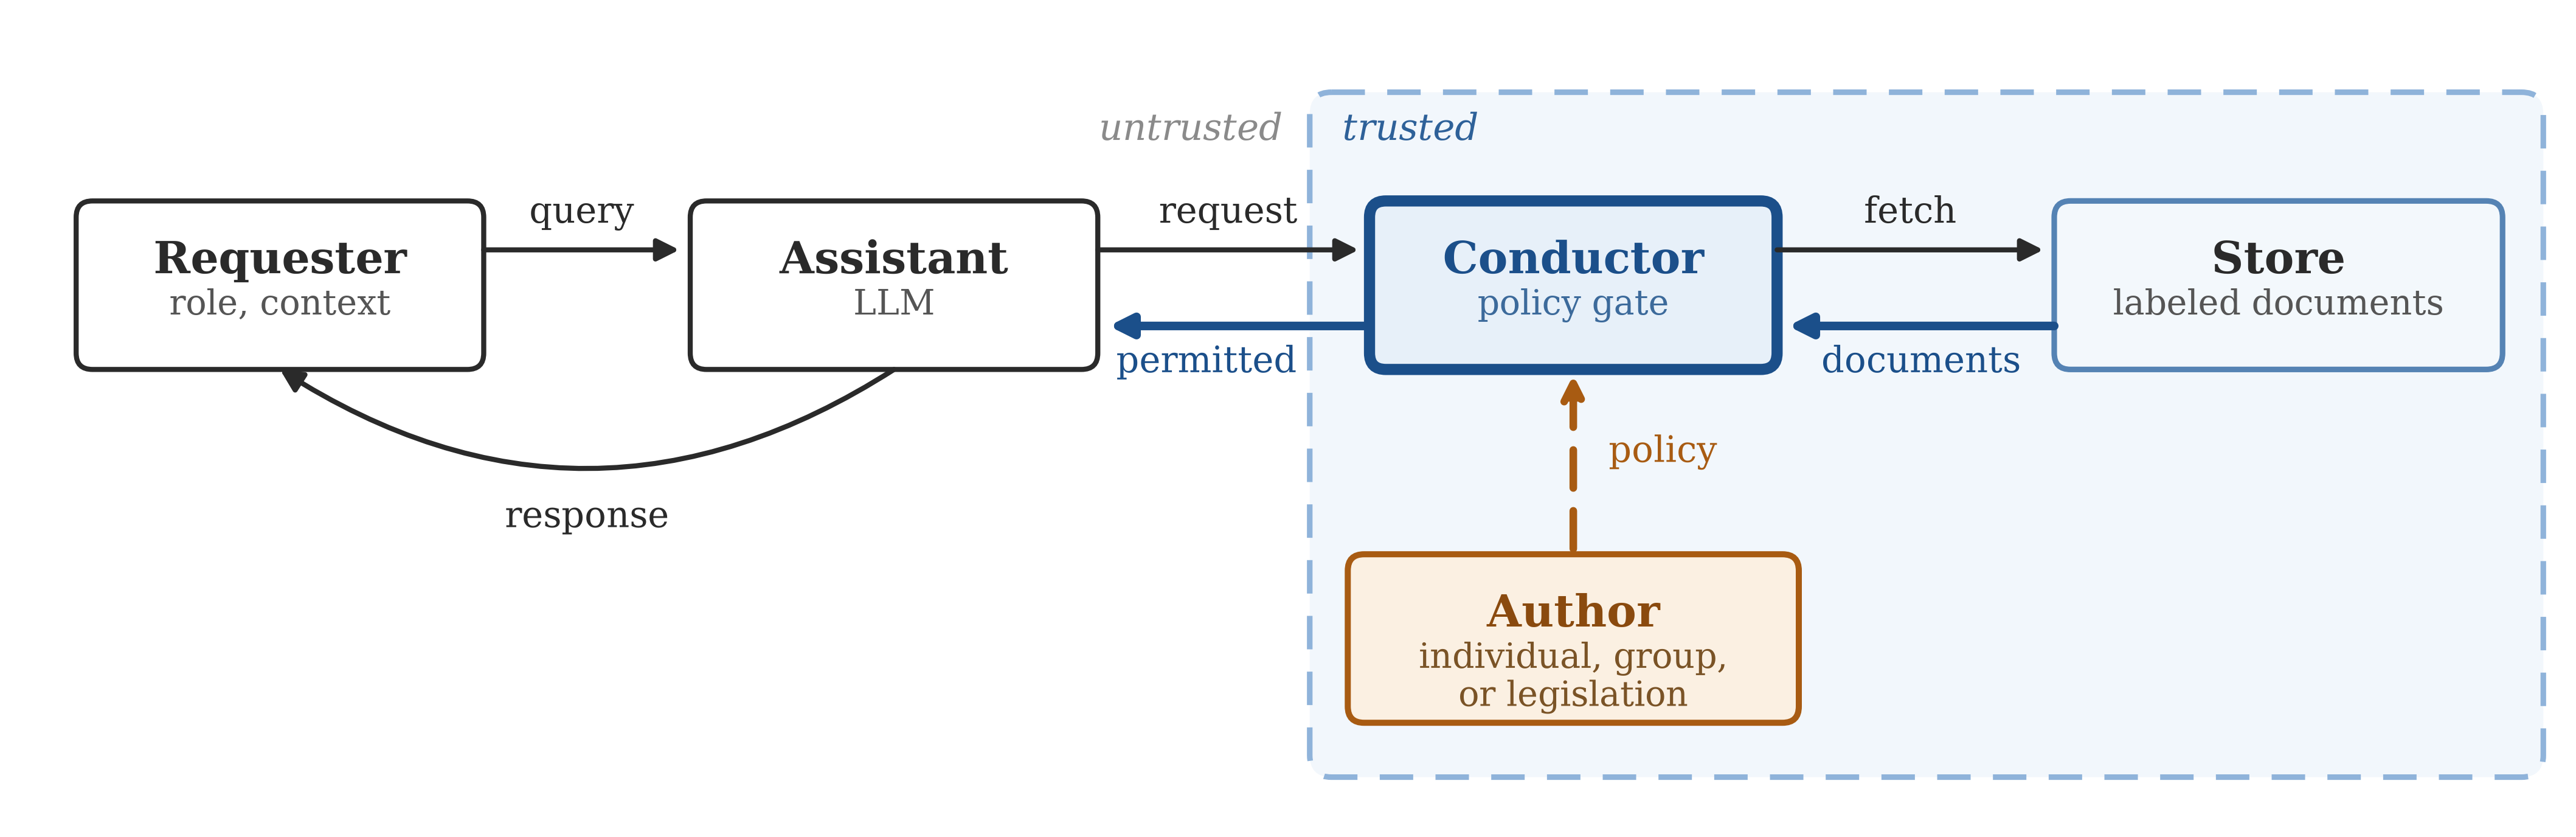
\includegraphics[width=\textwidth]{figures/conductor-architecture.png}}
\caption{The gated retrieval channel. The language model is treated as
trust-equivalent to the human requester: the gate sits inside the retrieval
tool, between the model and the record store, and returns either the document or
a denial. This work adds the information-type check as a fifth conjoined term,
leaving the channel's content-blindness intact.}
\label{fig:arch}
\end{figure*}

\subsection{The baseline gate}
The existing gate \cite{b4} applies four conjoined checks, shown as lines 1 to 4
of Fig.~\ref{fig:alg}, inside the retrieval channel of Fig.~\ref{fig:arch}. It
reads the requester's active role, that role's context, the document's label,
and whether the requester holds an assignment to the document's subject. It
never reads document content. On this corpus it permits 259 of 2520 flows.

\begin{figure}[t]
\hrule
\vspace{2pt}
\textbf{Algorithm 1} Extended gate. Lines 1--4 are the baseline, unmodified;
line 5 is this work.
\vspace{2pt}
\hrule
\vspace{3pt}
\begin{algorithmic}[1]
\STATE \textbf{require} requester $r$, document $d$, permissions $P$, types $T$
\IF{$\mathrm{activeRole}(r) = \bot$} \RETURN DENY \ENDIF
\IF{$\mathrm{context}(r) \neq \mathrm{authoritative}(\mathrm{role}(r))$}
    \RETURN DENY \ENDIF
\IF{$\mathrm{role}(r) \notin d.\mathrm{permittedRoles}$} \RETURN DENY \ENDIF
\IF{$\mathrm{tier}(d)$ needs assignment $\wedge\ \neg\mathrm{assigned}(r,
    \mathrm{subject}(d))$} \RETURN DENY \ENDIF
\STATE $E \leftarrow \{\, t \in T(d) : \mathrm{subj}(t,d) \,\} \setminus
    P(\mathrm{role}(r))$
\IF{$E \neq \emptyset$} \RETURN DENY, naming $E$ \ENDIF
\RETURN PERMIT
\end{algorithmic}
\vspace{2pt}
\hrule
\caption{}
\label{fig:alg}
\end{figure}

\section{Method}

\subsection{Controlled vocabulary}
Both sides of \eqref{eq:check} must be drawn from one enumerated set. We define
a 16-entry controlled vocabulary spanning four families: identity (name, date of
birth, Social Security Number, home address, emergency contact), clinical
(diagnosis, medication, history, mental health), financial (billing code,
insurance information), and employment (salary, employment contract, contract
terms, job title, medical licence). The vocabulary is a strict superset of the
label schema's existing attribute constants, so stored labels are valid
vocabulary members with no translation layer. It is versioned and
additive-only, and was frozen before permission authoring began.

An earlier tagger from prior work \cite{b28} could not supply this. Its
categories derive from a consumer profile schema and cover none of the clinical,
coding, insurance, or contract families; 9 of our 16 entries have no
counterpart. It is also architecturally a verifier, confirming which of a
supplied set of known values appear in a text, with no open-text detection path.
We therefore implemented a separate domain tagger.

\subsection{Tagger and audit}
\label{sec:tagger}
The tagger applies 37 deterministic rules, comprising structural patterns for
coded fields such as diagnosis codes, procedure codes, provider identifiers, and
masked Social Security Numbers, together with gazetteers for medications,
conditions, payers, and titles. It reads document text only and never reads the
label.

A stratified sample of 25 documents, drawn under a fixed seed with every tier
censused and all 21 document types covered, yields 400 document-type cells. The
annotator marks each type present or absent independently of what the tagger
reported, giving a full confusion matrix rather than a detections-only sheet, so
that recall, the direction that fails silently, is computable.

\subsection{Subject-linkage classification}
\label{sec:linkage}
Contextual Integrity defines the information type relative to the data subject.
A clinician's name in a signature block is not something \eqref{eq:check} should
govern: if a signature causes a document to carry the medical licence type, and
billing specialists may not receive that type, the gate would refuse an
insurance claim because a doctor signed it.

We classify each of the 1392 detections per occurrence as subject, third party,
organizational, or ambiguous. Ownership is resolved in two steps. A signal
yields an ownership role, one of subject-of-record, staff, other person, or
institution, which is then resolved against the document's subject type. This
makes the employment inversion fall out as a consequence rather than a special
case: where the subject is an employee, a clinician's name, title, licence, and
salary are subject-linked. Signals in priority order are vocabulary definition,
for entries that are subject-linked by definition; field label; section header;
name comparison against the document's subject; provider-block inheritance;
region; and a family default conditioned on subject type. No language model is
used at any point.

For the audit, 487 detections were annotated: every detection in the 25 audit
documents, giving 311 rows, plus every remaining third-party or organizational
detection corpus-wide, giving 176. The second block makes the union a census of
all filtered detections, so precision on the filtered classes is exact rather
than estimated. That is the priority quantity, because a detection wrongly
filtered out leaves the inventory entirely, so \eqref{eq:check} can never govern
it, the document is released, and nothing records that it happened. The
classifier's call was withheld from the review sheet to collect judgement rather
than confirmation.

\subsection{Authoring the role permission sets}
\label{sec:authoring}
The six permission sets are the normative artifact of this work and were
authored by the researcher. No model proposed, ranked, defaulted, or confirmed
any of the 96 decisions.

To make that authorship tractable without contaminating it, a template was
emitted with every cell blank: no recommended column, no default, and no
per-role-per-type statistic, since a per-cell count would be the outcome of that
cell's decision rather than an input to it. Each row carried the type's
definition verbatim, the number of documents carrying it as subject-linked, the
tier distribution, two example values, and the count of currently permitted
flows carrying it, all reported per type. A validator then required every cell
to hold a recognised value, so that blanks and typographical errors both fail
and a mistyped cell cannot become a silent denial, and checked vocabulary
membership in both directions.

The resulting sets are shown in Table~\ref{tab:perms}, and a written rationale
for each of the 96 decisions is released with the artifacts, including the
regulatory grounds where they apply and an explicit marking of the decisions
this corpus never exercises. The resulting sets are not otherwise defended here:
the argument of this paper is that a human must author them, not that this
particular authoring is correct. Two rows are worth flagging now because they
drive the results. The Social Security Number type is
the only fully locked row, permitted to the Patient role alone; and the job title
type is the only row permitted to every role, so \eqref{eq:check} never fires on
it and the effective vocabulary for the check is 15 of 16 entries. Validation
surfaced both shapes for confirmation before adjudication, and the author
confirmed them as intended.

\begin{table}[htbp]
\caption{Authored Role Permission Sets}
\begin{center}
\begin{tabular}{|l|c|c|c|c|c|c|}
\hline
\textbf{Information type}&\textbf{D}&\textbf{N}&\textbf{B}&\textbf{H}&\textbf{I}&\textbf{P} \\
\hline
Name & $\bullet$ & $\bullet$ & $\bullet$ & & & $\bullet$ \\
\hline
Date of birth & $\bullet$ & $\bullet$ & $\bullet$ & & & $\bullet$ \\
\hline
Social Security Number & & & & & & $\bullet$ \\
\hline
Home address & $\bullet$ & $\bullet$ & $\bullet$ & & & $\bullet$ \\
\hline
Emergency contact & $\bullet$ & $\bullet$ & & $\bullet$ & & $\bullet$ \\
\hline
Diagnosis & $\bullet$ & $\bullet$ & & & & $\bullet$ \\
\hline
Medication & $\bullet$ & $\bullet$ & & & & $\bullet$ \\
\hline
History & $\bullet$ & $\bullet$ & & & & $\bullet$ \\
\hline
Mental health$^{\mathrm{a}}$ & $\bullet$ & & & & & $\bullet$ \\
\hline
Billing code & $\bullet$ & $\bullet$ & $\bullet$ & & & $\bullet$ \\
\hline
Insurance information & $\bullet$ & $\bullet$ & $\bullet$ & & & $\bullet$ \\
\hline
Salary & $\bullet$ & $\bullet$ & $\bullet$ & $\bullet$ & & \\
\hline
Employment contract & $\bullet$ & $\bullet$ & $\bullet$ & $\bullet$ & $\bullet$ & \\
\hline
Contract terms & $\bullet$ & $\bullet$ & $\bullet$ & $\bullet$ & $\bullet$ & \\
\hline
Job title & $\bullet$ & $\bullet$ & $\bullet$ & $\bullet$ & $\bullet$ & $\bullet$ \\
\hline
Medical licence & $\bullet$ & $\bullet$ & $\bullet$ & $\bullet$ & & $\bullet$ \\
\hline
\textbf{Total permitted} & 15 & 14 & 10 & 6 & 3 & 13 \\
\hline
\multicolumn{7}{l}{D Doctor, N Nurse, B Billing Specialist, H HR Manager,} \\
\multicolumn{7}{l}{I IT Contractor, P Patient. $\bullet$ denotes permit.} \\
\multicolumn{7}{l}{$^{\mathrm{a}}$Extra-sensitive under the existing tier scheme.} \\
\end{tabular}
\label{tab:perms}
\end{center}
\end{table}

\subsection{The fifth check and its properties}
The extended gate calls the baseline gate unmodified and applies
\eqref{eq:check} only where the baseline permitted. Three properties are
verified empirically rather than asserted.

The check is \emph{monotone}: the extended permit set must be a subset of the
baseline permit set over all 2520 flows. Adjudication halts rather than
proceeding if this fails.

The check is \emph{content-free}: every flow is re-adjudicated with document
content and every attribute value replaced by a poison string, and decisions and
reason strings must be byte-identical. This substitutes a string that would
change any decision reading it, rather than merely inspecting the code path.

The check is \emph{stateless}: the full adjudication is re-run in a shuffled
order under a fixed seed, and per-flow results must be identical.

Denials name the triggering type, for example that role Doctor may not receive
the Social Security Number type about a named subject, carried by a clinical
note record. Without this, the new failure mode, a document refused because of
one attribute among eleven, would be opaque exactly where opacity is most
expensive.

\section{Results}

\subsection{Reconciliation: labels state purpose, not contents}
\label{sec:recon}
The tagger finds 801 document-type pairs across 1392 detections; the labels
author 291. No document of 105 matches its label exactly, with a mean Jaccard
similarity of 0.325. The asymmetry is the finding: only 10 authored pairs go
unconfirmed, while 520 pairs are present in content and claimed by no label, two
thirds of them independently corroborated by the generating model's own
extraction.

Two cases carry the argument. The Social Security Number type is authored on
zero of the 105 labels and present in 44 documents, all 44 corroborated. The
billing code type is authored on 18 documents and present in 65. Under the
baseline gate these travel with no field in the schema recording that they are
travelling.

\subsection{Tagger accuracy}
Across 400 annotated cells, precision is 0.994 with a 95 percent Wilson interval
of [0.969, 0.999], recall is 1.000 with interval [0.979, 1.000], and the miss
rate is 0.000, on a corpus five of the tagger's rules were revised against, so
these figures are an upper bound rather than a field estimate. Zero misses
across 177 present cells is the result that matters, because a miss means a type
never enters the inventory and \eqref{eq:check} cannot govern it. The single
false positive is an insurance-information detection arising from a gazetteer
matching a payer name in running prose. Per-type intervals are wide for rare
types; the contract-terms type rests on a single present cell, with a recall
interval of [0.21, 1.00].

\subsection{Linkage accuracy}
Of 1392 detections, 1229 (88.3 percent) are subject-linked, 137 (9.8 percent)
third party, 20 (1.4 percent) organizational, and 6 (0.4 percent) ambiguous.
Applying the classification to the reconciliation reduces the 520 unlabelled
pairs to 459 subject-linked, a 12 percent correction concentrated on job title,
medical licence, and name, the three types a signature block contaminates.

The human pass found and drove the repair of a defect. An organisation-name line
in the letterhead matched the section-header pattern and, because section scope
persisted forward without limit, governed entire documents in the nine cases
where no later header intervened, filtering clinical content as institutional.
Repairing it moved precision on the filtered classes from 0.704 to 0.955 and
recall on the subject class from 0.776 to 0.963, and reduced silent releases
from 66 to 6. The same human labels scored both versions and no re-annotation
was required, because the labels record ground truth independently of the
classifier.

\subsection{Over-delivery closed}
The check converts 81 of 259 permitted flows, or 31.3 percent, from permit to
deny, as shown in Table~\ref{tab:closed}. Monotonicity, content-freedom, and
statelessness all hold with zero violations over 2520 flows.

\begin{table}[htbp]
\caption{Over-Delivery Closed, by Responsible Information Type}
\begin{center}
\begin{tabular}{|l|c|c|}
\hline
\textbf{Information type}&\textbf{Flows}&\textbf{Sole cause} \\
\hline
Social Security Number & 57 & 36 \\
\hline
Medical diagnosis & 24 & 2 \\
\hline
Medical medication & 18 & 0 \\
\hline
Date of birth & 18 & 0 \\
\hline
Home address & 18 & 0 \\
\hline
Name & 14 & 0 \\
\hline
Mental health & 7 & 0 \\
\hline
Emergency contact & 5 & 0 \\
\hline
Medical history & 4 & 0 \\
\hline
\multicolumn{3}{l}{$^{\mathrm{a}}$By role: Billing 25, Doctor 24, HR 18, Nurse 14.} \\
\multicolumn{3}{l}{$^{\mathrm{b}}$By tier: financial 31, clinical standard 25,} \\
\multicolumn{3}{l}{employment 18, clinical sensitive 7.} \\
\end{tabular}
\label{tab:closed}
\end{center}
\end{table}

The motivating example reproduces exactly. Insurance claims are correctly
released to billing specialists by the role check, and the diagnosis printed on
them is now refused: 24 flows, concentrated on insurance claims and billing
statements.

\subsection{Over-blocks introduced}
Over-blocks are norm violations too and are reported separately, never netted
against the closures. They are measured, not asserted. The check is re-run with
subject linkage taken from the human labels instead of the classifier, on the 25
documents where every detection carries a label. Flows that flip back to permit
under ground truth are denials caused by linkage error rather than by policy.

The result is zero over-blocks across 600 flows, of which 16 were check-five
denials. The detector was proved capable of firing: a synthetic correction
removing the Social Security Number type from those documents makes it report
six. Five of the 25 documents do have differing type sets under human labels,
but none changes a decision. This is a real result with narrow support, and the
scope should travel with it.

\subsection{Denial overlap and the role-field ablation}
\label{sec:overlap}
Of 2342 denials, 1054 are role-only, 840 are caught by both the role and the
attribute check, 219 by the attribute check together with another check, 148 by
another check alone, and 81 are attribute-only. That last set is exactly the
closed set, and it is disjoint from anything the baseline could reach.

Removing the permitted-roles field entirely, so that every role is permitted on
every document, raises permits from 259 to 427 under four checks and from 178 to
278 under five. The role field therefore uniquely blocks 100 flows that the type
check does not catch, 90 of them on internal-tier documents. Internal documents
such as staff schedules, meeting agendas, and policy memoranda carry almost no
subject-linked types, so the type check has nothing to test and passes them
freely.

The two fields are therefore non-redundant in both directions. The role field
governs documents by what they are, the type check by what they contain, and a
document with no governable contents is invisible to the second.

\subsection{Unreachable documents}
\label{sec:unreachable}
67 of 105 documents become reachable by no one, because every role their label
admits is refused by \eqref{eq:check}. Reachable documents fall from 87 to 27.
Of these, 22 are blocked by the Social Security Number type alone and the rest
by combinations, as shown in Table~\ref{tab:unreach}. One insurance claim admits
only the Billing Specialist role while carrying emergency contact, diagnosis,
history, medication, and Social Security Number, five types that role may not
receive.

\begin{table}[htbp]
\caption{Unreachable Documents by Blocking Type Set}
\begin{center}
\begin{tabular}{|l|c|}
\hline
\textbf{Blocking types}&\textbf{Documents} \\
\hline
Social Security Number alone & 22 \\
\hline
Date of birth, home address, name & 12 \\
\hline
Diagnosis, medication, SSN & 7 \\
\hline
Diagnosis, SSN & 5 \\
\hline
Mental health, SSN & 3 \\
\hline
Other combinations & 18 \\
\hline
\multicolumn{2}{l}{$^{\mathrm{a}}$Tiers: financial 24, clinical standard 18,} \\
\multicolumn{2}{l}{employment 18, clinical sensitive 7.} \\
\end{tabular}
\label{tab:unreach}
\end{center}
\end{table}

\subsection{A bound on the mechanism}
\label{sec:bound}
A document is reachable if and only if some admitted role covers its whole
bundle:
\begin{equation}
\mathrm{unreachable}(d) \iff \forall r \in R(d):\ T(d) \setminus P(r) \neq
\emptyset .
\label{eq:unreach}
\end{equation}
Note what \eqref{eq:unreach} is not. It is not $T(d) \subseteq \bigcup_{r} P(r)$.
Coverage does not compose across roles, because a document is released to one
requester at a time. Two roles that jointly cover a bundle still leave it
unreachable if neither covers it alone. This is the formal reason the result is
a property of document-level enforcement rather than of any particular policy.

Under a null model in which $T(d)$ is a uniform random $k$-subset of the
vocabulary $V$, coverage is hypergeometric,
\begin{equation}
\Pr[T \subseteq P(r)] = \binom{|P(r)|}{k} \Big/ \binom{|V|}{k},
\label{eq:cover}
\end{equation}
which behaves like $p^{k}$, so coverage decays exponentially in bundle size.
Fig.~\ref{fig:coverage} plots \eqref{eq:cover} for each authored permission set.
Critical bundle sizes, meaning the largest $k$ at which a random bundle is still
more likely than not to be covered, are 8 for Doctor, 4 for Nurse, 3 for
Patient, 1 for Billing Specialist, and 0 for HR Manager and IT Contractor. The
shaded region marks the bundle sizes this corpus actually exhibits, from 4 to
11: by the time a document carries the mean of 7.67 types, only the Doctor role
retains better than even odds of covering it, and the three administrative roles
have fallen effectively to zero.

\begin{figure}[htbp]
\centerline{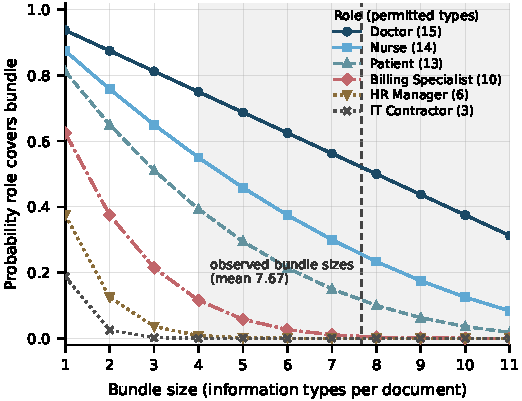
\includegraphics[width=\columnwidth]{figures/coverage-curve.pdf}}
\caption{Probability that a role covers a random bundle of $k$ information
types, from \eqref{eq:cover}, with each role's permitted-type count in
parentheses. Coverage decays exponentially in bundle size. The shaded region is
the bundle-size range observed in this corpus; the dashed line is its mean.}
\label{fig:coverage}
\end{figure}

Instantiating this as a test rather than a fit, holding the authored permission
sets, the admitted role sets, and the bundle-size distribution fixed and
randomising only which types each bundle contains, the model predicts 66.01
unreachable documents against 67 observed, a discrepancy of $+0.99$.

The aggregate agreement is partly cancellation, and we report that rather than
resting on it. The sum of absolute per-stratum deviations is 15.91, with the
model under-predicting at $k=6$ and $k=7$ and over-predicting at $k=9$ and
$k=10$. The driver is identified: the Social Security Number type appears in
90.9 percent of bundles with $k \geq 9$ against a base rate of 46.3 percent, and
the Patient role, its only permitted role, is admitted on none of those
documents. Real large bundles are systematically less coverable than random
ones, so the null model's one assumption, content independence, is violated in a
direction that matters.

\section{Discussion}

\subsection{What over-delivery costs}
The 81 closed flows are not policy errors in the baseline gate. Every one passed
role, context, and assignment correctly, and the documents were released to
requesters entitled to them. What travelled alongside was never represented in
the decision. The dominant contributor, the Social Security Number type, is
instructive: it appears on no label, so no amount of care in authoring the
permitted-roles field could have governed it. The schema recorded a field that
the enforcement path never read, and the information moved.

This is the practical content of the granularity mismatch. Enforcement at the
object delivers the object's contents, and unless those contents are enumerated
somewhere the decision procedure consults, they are ungoverned by construction
rather than by oversight.

\subsection{Why the two fields do not subsume each other}
Section~\ref{sec:overlap} measures rather than argues this. The type check
catches 81 flows the role field misses; the role field catches 100 the type
check misses, 90 of them on internal-tier documents that carry almost no
subject-linked information at all. A staff schedule is not sensitive because of
the attributes it contains, since it contains almost none, but because of what
it is and who should see it.

The implication for design is that attribute-level policy is a complement to
object-level policy, not a replacement. A system that discarded the
permitted-roles field in favour of information-type permissions would open 100
flows on this corpus. Both terms of the conjunction earn their place.

\subsection{The limit of content-blind enforcement}
\label{sec:limit}
Section~\ref{sec:unreachable} is the most consequential result and the one most
easily mis-stated. The 67 unreachable documents are not a malfunction. Each is
refused because its label admits only roles that cannot lawfully receive
everything it contains, and \eqref{eq:check} is the first mechanism in the
pipeline able to notice.

Specification-first labelling produces documents whose contents exceed what any
admitted role may lawfully receive; in this corpus that affects 64 percent of
documents. The mechanism generalizes, as Section~\ref{sec:bound} shows by
deriving it from bundle size against permission-set size with no appeal to this
corpus's particulars, but the magnitude does not, and depends on how the corpus
was built.

The remedy is outside what this gate can do. Making an unreachable document
reachable requires removing types from it, by redaction or by decomposition into
several narrower documents. Both require reading and rewriting content, and the
gate's content-blindness, verified earlier and the property that makes it
trustworthy against prompt injection, is exactly what prevents it. A
content-blind gate can detect that a document should not exist in its current
form; it cannot fix it.

\subsection{Normative authorship}
Prior work \cite{b4} found language models unable to author policy of this kind
reliably. That constrained the design here: the 96 permission decisions were
made by hand, and the tooling was built to keep them uncontaminated, with blank
cells, no recommendations, and per-type rather than per-cell impact figures.

The cost is real. 96 decisions is tractable; a feasibility assessment for the
external corpus discussed in Section~\ref{sec:threats} estimates roughly 350
further mapping judgements, each of which is normative rather than clerical.
Attribute-level enforcement does not remove human normative work. It relocates
it from per-document labelling to per-role-per-type policy, where it is at least
reusable across documents.

\subsection{The type boundary is not inference-proof}
The billing code type is permitted to the Billing Specialist role while the
diagnosis type is denied, yet the same diagnosis code can instantiate either,
separated by document context rather than by value. A billing specialist denied
the stated diagnosis may still receive the identical code. The existing policy
module has recorded that implication since prior work, and \eqref{eq:check} does
not consult it. The protection here is procedural, not semantic, and the 24
flows closed on the diagnosis type should be read with that bound attached.

\section{Threats to Validity}
\label{sec:threats}

The corpus is synthetic and was built by us, specification-first, which is
precisely the condition Section~\ref{sec:limit} identifies as producing
unreachable documents. A corpus whose labels were derived from content would
show fewer. The derived bound of Section~\ref{sec:bound} is the response: it
makes the mechanism a claim about bundle size and permission overlap rather than
about these 105 documents.

External validation is not available in the form needed. We examined the health
privacy split of PrivaCI-Bench \cite{b26}, comprising 214 court-derived flows,
whose label authority is external. Every flow carries exactly one information
type, so the bundling mechanism this work measures is structurally absent; there
is also no document layer, no tier, and no assignment relation. Only 107 of the
214 flows carry a usable expected decision, of which 20 are negative. It could
validate the permission sets, a narrower and still useful claim, but it cannot
test the fifth check as such.

Measurement inherits extraction error. All adjudication figures rest on the
tagger and the linkage classifier. The tagger is audited at 0.994 precision and
1.000 recall, but on a corpus five of its rules were revised against, and with
wide intervals for rare types. The linkage classifier is audited at 0.955
precision on the filtered classes and 0.963 recall on the subject class, with
six residual silent releases corpus-wide.

Annotation used a single annotator, with no adjudication and no inter-rater
agreement. The reviewer was instructed to prefer the subject or ambiguous label
under uncertainty, so reported precision on the filtered classes is conservative
against our own finding rather than flattering to it.

The over-block figure covers 600 of 2520 flows, containing 16 check-five
denials. It establishes that linkage error had no policy consequence on that
scope; it does not establish this for the remaining flows, where no ground truth
exists.

Finally, the permission sets reflect one author's normative judgement, with no
second authority and no inter-rater measurement. That is the correct provenance
for the argument, which is that a human must author them, but the 81 closed
flows and 67 unreachable documents follow from one normative reading rather than
a validated one.

\section{Future Work}

Four directions follow directly from the limits identified above.

\textbf{Closing the inference gap between types.} The billing code and diagnosis
types are separated by document context rather than by value, so a role denied
one may receive the same code through the other. Two remedies are available and
neither is free. Propagating the implication relation through \eqref{eq:check},
so that permitting an implying type entails permitting what it implies, would
make some authored cells mutually inconsistent and force re-authoring. Splitting
the billing code type into procedure and diagnosis codes would change a frozen
vocabulary and invalidate the permission sets keyed against it. Which is
preferable is an empirical question about how often the implication is
exploitable in practice, and we have not measured that.

\textbf{Redaction and decomposition as first-class operations.}
Section~\ref{sec:limit} shows a content-blind gate can detect that a document
should not exist in its current form but cannot repair it. The natural extension
is a separate, content-reading component that proposes redactions or
decompositions, kept architecturally distinct from the gate so that the gate's
content-blindness is preserved. The interesting question is the trust boundary:
such a component reads content and therefore reopens the injection surface the
gated design was built to close, so it would have to be positioned outside the
decision path, with the gate still adjudicating the resulting narrower documents.

\textbf{Multi-subject documents.} Our treatment of the emergency contact type
resolves it as an attribute of the subject, on the grounds that the designation
is a relational fact about them. That is defensible for the subject and leaves
the contact, a real person who consented to nothing, with their identity and
telephone number governed entirely by the subject's permissions. Family history
has the same shape. The gate assumes one subject per document while Contextual
Integrity requires no such thing, and representing a subject per information
type rather than per document would require changes to the label, the assignment
relation, and the check together.

\textbf{External and document-level corpora.} The corpus property this work
needs is narrow: documents bundling multiple typed attributes under role-scoped
release rules. Existing Contextual Integrity benchmarks do not supply it, as
Section~\ref{sec:threats} records, so a clinical records benchmark may serve
better than a privacy benchmark. Absent such a corpus, the bound of
Section~\ref{sec:bound} carries the generalization claim, and a study that
varied bundle size and permission-set size independently, even synthetically,
would test it more sharply than this corpus can.

\section{Conclusion}

Contextual Integrity is defined over information types; deployed access control
enforces over objects. We measured what that mismatch costs on a system whose
object-level policy is otherwise correct, by adding a fifth conjoined check
requiring a document's subject-linked information types to be a subset of those
its recipient's role may receive.

Supporting the check required building and auditing the inventory the system
lacked, and the audit was not a formality. It found a classifier defect that had
been silently filtering clinical content as institutional, and repairing it moved
precision on the filtered classes from 0.704 to 0.955. Reconciling the finished
inventory against the hand-authored labels, no document of 105 matched exactly,
and 520 document-type pairs, 459 of them subject-linked, were present but
unlabelled.

The check closes 81 of 259 permitted flows with zero over-blocks across the 600
flows where ground truth exists, while remaining monotone, content-free, and
stateless. It does not subsume the object-level role check, which uniquely
blocks 100 flows of its own. And it surfaces a limit: 67 of 105 documents become
reachable by nobody, because specification-first labelling produces documents
whose contents exceed what any admitted role may lawfully receive. A derived
bound predicts that figure to within one document and identifies bundle size as
the governing parameter. The mechanism generalizes; the magnitude does not.

A content-blind gate can determine that a document should not exist in its
current form. Fixing it, by redaction or decomposition, requires reading
content, which is exactly what such a gate must not do.

\section*{Reproducibility}

All artifacts are deterministic and byte-identical on re-run, and every stage
verifies a corpus hash before executing. Annotation sheets, the authored
permission sets and their written rationale, per-flow adjudications, and the
derivation are released alongside the code.

\begin{thebibliography}{00}
\bibitem{b1} H. Nissenbaum, Privacy in Context: Technology, Policy, and the Integrity of Social Life. Stanford, CA: Stanford University Press, 2010.
\bibitem{b2} A. Barth, A. Datta, J. C. Mitchell, and H. Nissenbaum, ``Privacy and contextual integrity: Framework and applications,'' in Proc. IEEE Symp. Security and Privacy, 2006, pp. 184--198.
\bibitem{b3} R. S. Sandhu, E. J. Coyne, H. L. Feinstein, and C. E. Youman, ``Role-based access control models,'' IEEE Computer, vol. 29, no. 2, pp. 38--47, 1996.
\bibitem{b4} R. Thornton, ``Privacy conductor: A deterministic contextual integrity gate for language model document retrieval,'' unpublished.
\bibitem{b5} K. Martin and H. Nissenbaum, ``Measuring privacy: An empirical test using context to expose confounding variables,'' Columbia Science and Technology Law Review, vol. 18, pp. 176--218, 2016.
\bibitem{b6} N. Apthorpe, Y. Shvartzshnaider, A. Mathur, D. Reisman, and N. Feamster, ``Discovering smart home Internet of Things privacy norms using contextual integrity,'' Proc. ACM on Interactive, Mobile, Wearable and Ubiquitous Technologies, vol. 2, no. 2, pp. 1--23, 2018.
\bibitem{b7} S. Benthall, S. Gurses, and H. Nissenbaum, ``Contextual integrity through the lens of computer science,'' Foundations and Trends in Privacy and Security, vol. 2, no. 1, pp. 1--69, 2017.
\bibitem{b8} S. D. Warren and L. D. Brandeis, ``The right to privacy,'' Harvard Law Review, vol. 4, no. 5, pp. 193--220, 1890.
\bibitem{b9} N. Carlini et al., ``Extracting training data from large language models,'' in Proc. 30th USENIX Security Symp., 2021, pp. 2633--2650.
\bibitem{b10} P. Lewis et al., ``Retrieval-augmented generation for knowledge-intensive natural language processing tasks,'' in Advances in Neural Information Processing Systems, 2020.
\bibitem{b11} T. Schick et al., ``Toolformer: Language models can teach themselves to use tools,'' in Advances in Neural Information Processing Systems, 2023.
\bibitem{b12} S. Yao et al., ``ReAct: Synergizing reasoning and acting in language models,'' in Proc. Int. Conf. Learning Representations, 2023.
\bibitem{b13} Y. Ruan et al., ``Identifying the risks of language model agents with a language model emulated sandbox,'' in Proc. Int. Conf. Learning Representations, 2024.
\bibitem{b14} F. Perez and I. Ribeiro, ``Ignore previous prompt: Attack techniques for language models,'' in NeurIPS Machine Learning Safety Workshop, 2022.
\bibitem{b15} K. Greshake, S. Abdelnabi, S. Mishra, C. Endres, T. Holz, and M. Fritz, ``Not what you've signed up for: Compromising real-world language model integrated applications with indirect prompt injection,'' in Proc. 16th ACM Workshop on Artificial Intelligence and Security, 2023, pp. 79--90.
\bibitem{b16} N. Mireshghallah et al., ``Can language models keep a secret? Testing privacy implications of language models via contextual integrity theory,'' in Proc. Int. Conf. Learning Representations, 2024.
\bibitem{b17} Y. Shao, T. Li, W. Shi, Y. Liu, and D. Yang, ``PrivacyLens: Evaluating privacy norm awareness of language models in action,'' in Advances in Neural Information Processing Systems Datasets and Benchmarks Track, 2024.
\bibitem{b18} E. Bagdasarian et al., ``AirGapAgent: Protecting privacy-conscious conversational agents,'' in Proc. ACM SIGSAC Conf. Computer and Communications Security, 2024.
\bibitem{b19} S. Ghalebikesabi et al., ``Operationalizing contextual integrity in privacy-conscious assistants,'' arXiv:2408.02373, 2024.
\bibitem{b20} V. C. Hu et al., ``Guide to attribute based access control (ABAC) definition and considerations,'' National Institute of Standards and Technology, NIST Special Publication 800-162, 2014.
\bibitem{b21} OASIS, ``eXtensible access control markup language (XACML) version 3.0,'' OASIS Standard, 2013.
\bibitem{b22} J.-W. Byun and N. Li, ``Purpose based access control for privacy protection in relational database systems,'' The VLDB Journal, vol. 17, no. 4, pp. 603--619, 2008.
\bibitem{b23} R. Agrawal, J. Kiernan, R. Srikant, and Y. Xu, ``Hippocratic databases,'' in Proc. 28th Int. Conf. Very Large Data Bases, 2002, pp. 143--154.
\bibitem{b24} O. Uzuner, Y. Luo, and P. Szolovits, ``Evaluating the state-of-the-art in automatic de-identification,'' Journal of the American Medical Informatics Association, vol. 14, no. 5, pp. 550--563, 2007.
\bibitem{b25} L. Sweeney, ``k-anonymity: A model for protecting privacy,'' International Journal of Uncertainty, Fuzziness and Knowledge-Based Systems, vol. 10, no. 5, pp. 557--570, 2002.
\bibitem{b26} H. Li, W. Hu, H. Jing, Y. Chen, Q. Hu, S. Han, T. Chu, P. Hu, and Y. Song, ``PrivaCI-Bench: Evaluating privacy with contextual integrity and legal compliance,'' in Proc. 63rd Annu. Meeting Assoc. Computational Linguistics, Vienna, Austria, 2025, pp. 10544--10559.
\bibitem{b27} W. Fan, H. Li, Z. Deng, W. Wang, and Y. Song, ``GoldCoin: Grounding large language models in privacy laws via contextual integrity theory,'' in Proc. Conf. Empirical Methods in Natural Language Processing, 2024.
\bibitem{b28} R. Thornton, ``PANOPTICON: A synthetic corpus of personally identifiable information laden prompts with span level ground truth,'' unpublished.
\end{thebibliography}

\end{document}
